\chapter{Συνδεσμολογία}

Κατά την εκκίνηση της συσκευής, δηλαδή κατά τη σύνδεσή της με την παροχή
τροφοδοσίας, εκτελείται η αρχικοποίηση των διαφόρων υποσυστημάτων της υλοποίησης
και, εν συνεχεία, ο μικροελεγκτής μεταπίπτει σε κατάσταση χαμηλής κατανάλωσης
ισχύος. Από αυτήν, ενεργοποιείται αυτόματα είτε για την εκκίνηση ενός νέου
κύκλου μετρήσεων (βλ. \nameref{sec:task} σ.~\pageref{sec:task}), είτε για την
εξυπηρέτηση κάποιου εισερχόμενου αιτήματος HTTP (βλ. \nameref{%
sec:network:impl-resources} σ.~\pageref{sec:network:impl-resources}). Στο σχήμα
\ref{fig:mcu:tasks} παρουσιάζεται ο κύκλος καθηκόντων του μικροελεγκτή.

\begin{figure}
    \caption{Καθήκοντα του μικροελεγκτή.\label{fig:mcu:tasks}}
    \begin{center}
    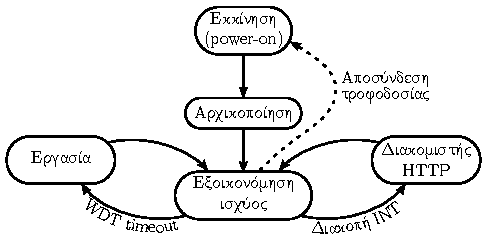
\includegraphics{mcu_tasks}
    \end{center}
\end{figure}

Αναλυτικότερα, κατά το στάδιο της αρχικοποίησης, τίθεται η συχνότητα του
ρολογιού του μικροελεκτή, η οποία, για τις ανάγκες της υλοποίησης, μειώνεται από
τα 16MHz στα 4MHz και η κατεύθυνση των ακροδεκτών (δηλαδή ποιοι είναι εισόδου
και ποιοι εξόδου). Επίσης, ρυθμίζεται το κύκλωμα WDT (\te{Watch-Dog Timer}), το
οποίο είναι υπεύθυνο για την περιοδική αφύπνιση του μικροελεγκτή ώστε να
ελέγχεται η ανάγκη εκκίνησης νέου κύκλου μετρήσεων.

Επιπλέον, ανακτώνται οι μεταβλητές ρυθμίσεις της συσκευής είτε από τις
προκαθορισμένες (εργοστασιακές ρυθμίσεις), είτε από τις αποθηκευμένες τιμές της
εφεδρικής μνήμης, εφόσον αυτές είναι έγκυρες (βλ \nameref{subsec:backup-memory}
σ.~\pageref{subsec:backup-memory}).
Οι ρυθμίσεις αυτές περιλαμβάνουν τη δικτύωση της συσκευής (διεύθυνση IP, μάσκα
υποδικτύου, προεπιλεγμένη πύλη), το λειτουργικό εύρος του υποσυστήματος κίνησης
(βλ. \nameref{sec:motor:coordinates} σ.~\pageref{sec:motor:coordinates}), το
χρονικό διάστημα μεταξύ κύκλων εργασίας καθώς και το πλήθος μετρήσεων που
πραγματοποιείται σε κάθε κύκλο (βλ. \nameref{sec:task} σ.~\pageref{sec:task}).
Ο τρόπος ρύθμισης της συσκευής περιγράφεται στους Πόρους υλοποίησης (σ.~%
\pageref{sec:network:impl-resources}).

Στην πορεία, οι ρυθμίσεις προωθούνται στις κατάλληλες μονάδες και εκτελούνται
επιπρόσθετες προετοιμασίες, όπως η παλιννόστηση της κεφαλής, δηλαδή η επαναφορά
της στη θέση επιστροφής (συντεταγμένες [0, 0, Z\tsub{max}]) (βλ. σ.~%
\pageref{sec:motor:homing}) και η αρχικοποίηση του HTTP \te{Socket} (βλ. σ.~%
\pageref{ssubsec:network:port_mr}).









